\lfoot{Autor: Daniel Melichar}
\subsubsection{Relationale Datenbanken}
\label{subsec:relationaleDB}

Die relationale Datenbank ist seit dem ersten Erscheinen in 1970 weit gekommen und ist von den meisten Großkonzernen der Welt adaptiert worden. Mit der eigens dafür entwickelten \textit{Programmiersprache} SQL (Structured Query Langauge) war das umgehen mit Datenbanken und Tabellen und der darin gespeicherten Information so einfach wie noch nie. Es ist zu beachten, dass es ein wenig mehr zu NoSQL Datenbanken gibt, da wir mit einer solchen arbeiten (siehe \ref{subsec:datenmanagementimpl})

\begin{figure}[!htb]\centering
	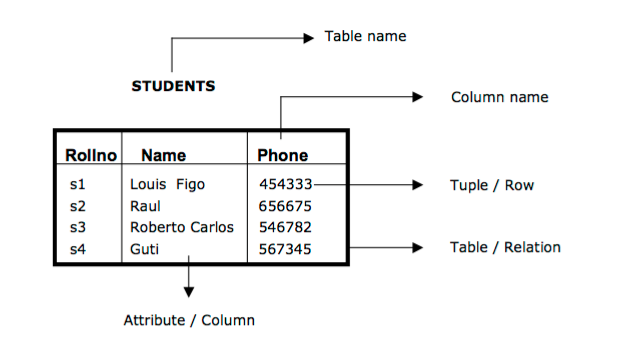
\includegraphics[width=0.8\textwidth]{images/relationaleTabelle}
	\caption{Beispiel einer relationalen Datenbank}
\end{figure}

Features von relationalen DBMS (Achtung: diese sind stark vom eigentlichem DBMS abhängig)
\begin{itemize}
\item Unterstützt eine große Menge an Daten
\item Datensicherheit durch backups, permissions, etc.
\item Fehler Toleranz und Wiederherstellung
\end{itemize}

Hinter den Kulissen sorgt das Relational Database Management System (RDBMS) dafür das die Eigenschaften des ACID (Atomicity, Consistency, Isolation, Durability) Prinzips der Transaktionen so funktionieren wie sie sollen. Beachtet man nun auch die anderen Features der Sprache, so wie Constraints (primary and foreign keys, Datentype, etc.) oder Stored Procedures/Functions, erkennt man schnell, dass je mehr Information eine relationale Datenbank enthält, desto langsamer wird sie.

Einige der größten Limitierungen \cite{MELD.CH2-relationaleDB.rdbmsBuch} durch das relationale Datenbank Model sind
\begin{itemize}
\item Skalierbarkeit: ab einem gewissen Zeitpunkt muss die Datenbank über mehrere Server laufen da ein Server nicht mehr genügend Ressourcen verfügt um die Daten zu managen
\item Komplexität: die Daten müssen zu Tabellen strukturiert werden; es ist also ein Schema notwendig
\item Features: Meist für Datenintegrität aber nicht für Datenverarbeitung 
\end{itemize}


Zusammenfassed kann man also sagen, dass die Verwendung eines RDBMS dann sinn macht, wenn man ein Datenschema erstellen kann. Das bedeutet konkret: wenn man weiß welche Daten man hat und haben wird, wie man diese in eine Tabellen Struktur einbauen kann, und man Anforderungen die sich nur im geringen Maß ändern können ist es sinnvoll ein RDBMS zu verwenden. Die zur Verfügung gestellten Features werden einen Administrator sehr gut unterstützen. 
\clearpage % DO NOT REMOVE